\par En ce qui concerne la duplication du prototype, il est en premier lieu important d'énoncer une liste complète de tous les composants utilisés :
\begin{itemize}
    \item un microcontrôleur (fourni par l'ULB dans ce cas) ;
    \item un moteur pas-à-pas 42SH38-4A ;
    \item un moteur pas-à-pas 17HS19-2004S1 (ainsi qu'un support de montage permettant de tenir le moteur horizontalement) ;
    \item deux drivers pour moteur pas-à-pas L293D ;
    \item un kit d'extrusion de la marque Redrex adapté à un moteur pas-à-pas NEMA 17 ;
    \item un servomoteur SG90 ;
    \item deux breadboards ;
    \item du fil électrique ;
    \item une pince à dénuder multi-fonctions (achetée via Cotubex) ;
    \item les pièces à imprimer en 3D mentionnées plus haut.
\end{itemize}

Le prototype final obtenu peut être visualisé ci-dessous :

\begin{figure}[H]
    \centering
    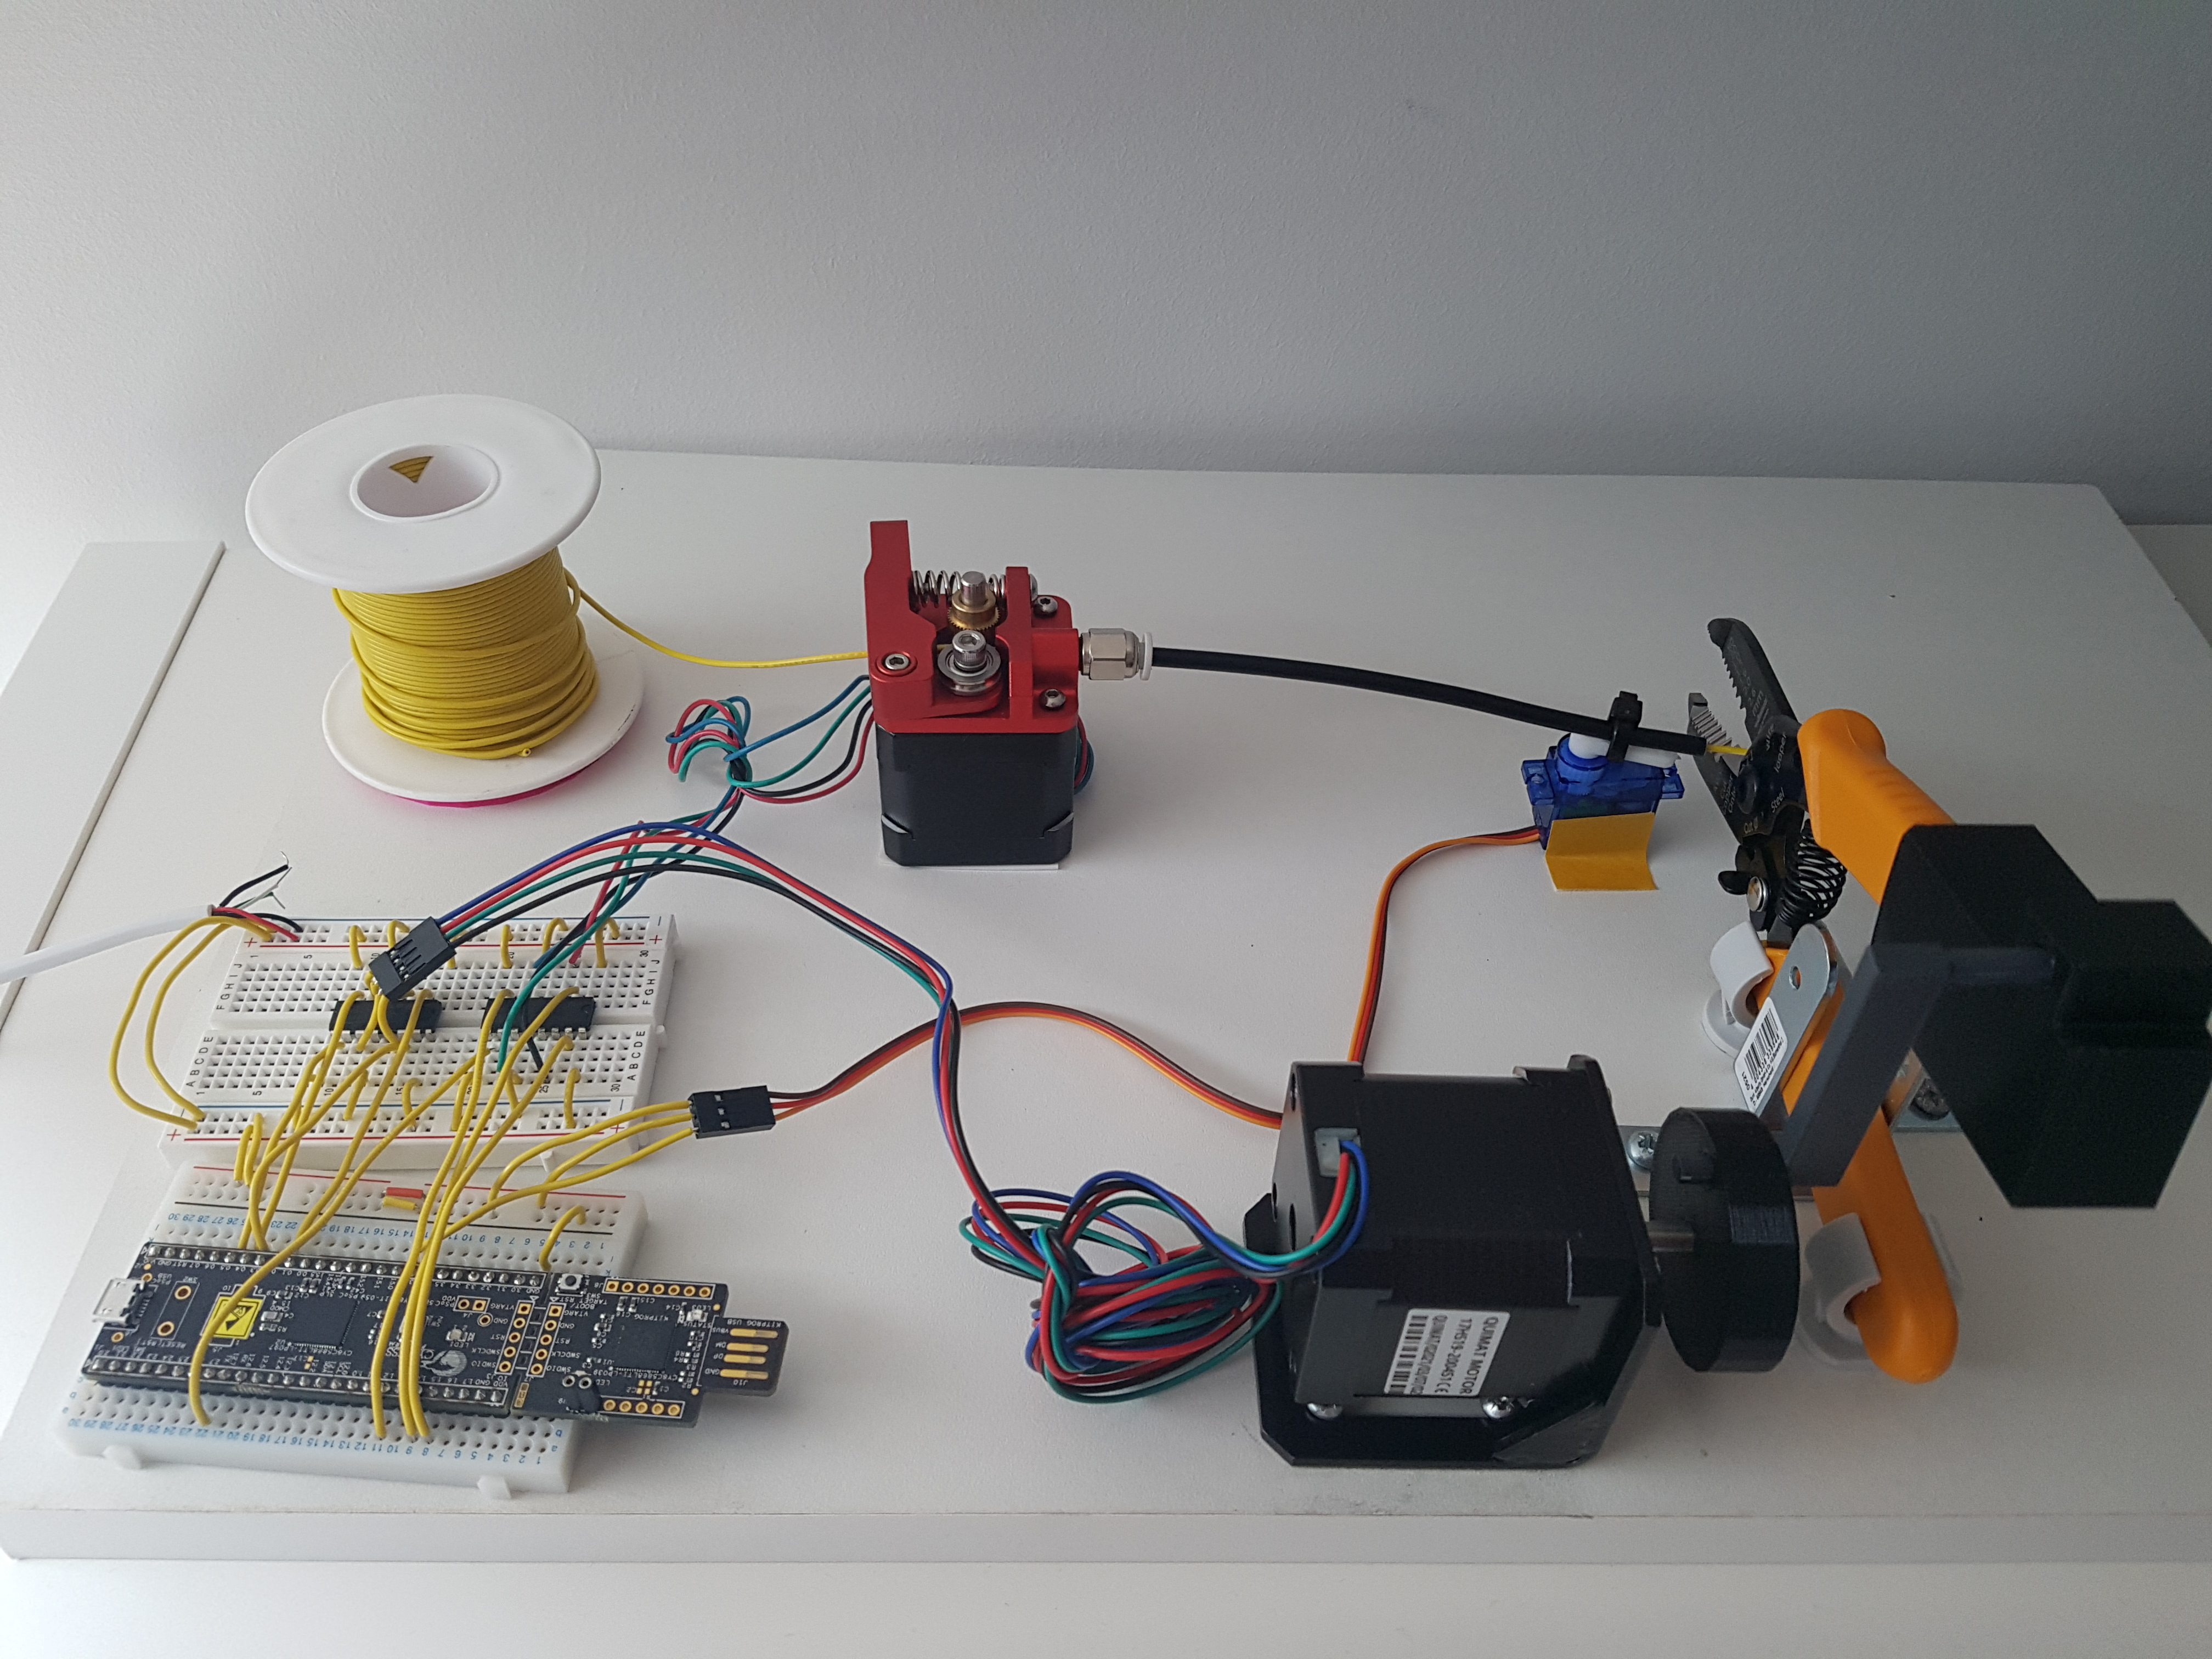
\includegraphics[width=0.65\textwidth]{images/proto1.jpg}
    \caption{Prototype final}
    \label{fig:proto1}
\end{figure}

\par Le circuit électrique se compose notamment du microcontrôleur connecté aux deux drivers de moteur pas-à-pas, eux-mêmes connectés aux moteurs de coupe et de tirage selon les connexions décrites dans les datasheets des composants.
\par Une bobine de fil électrique est liée au premier moteur pas-à-pas qui se charge du tirage ; le fil passe dans un tube dirigé par un servomoteur et est amené vers la pince à dénuder. Cette dernière est liée au deuxième moteur pas-à-pas par un système de bielle-manivelle construit à l'aide de pièces imprimées en 3D. Le tout tient sur une planche en bois.
\par À part les pièces mentionnés dans la liste plus haut, des pièces sont nécessaires pour construire le petit dispositif permettant de tenir la pince à dénuder verticalement. Ici, ce sont simplement des supports de construction utilisés : deux de forme circulaire pour assurer que la pince tient verticalement, et deux en forme d'angle perpendiculaire pour assurer que la pince ne se déloge pas horizontalement.

\begin{figure}[H]
    \centering
    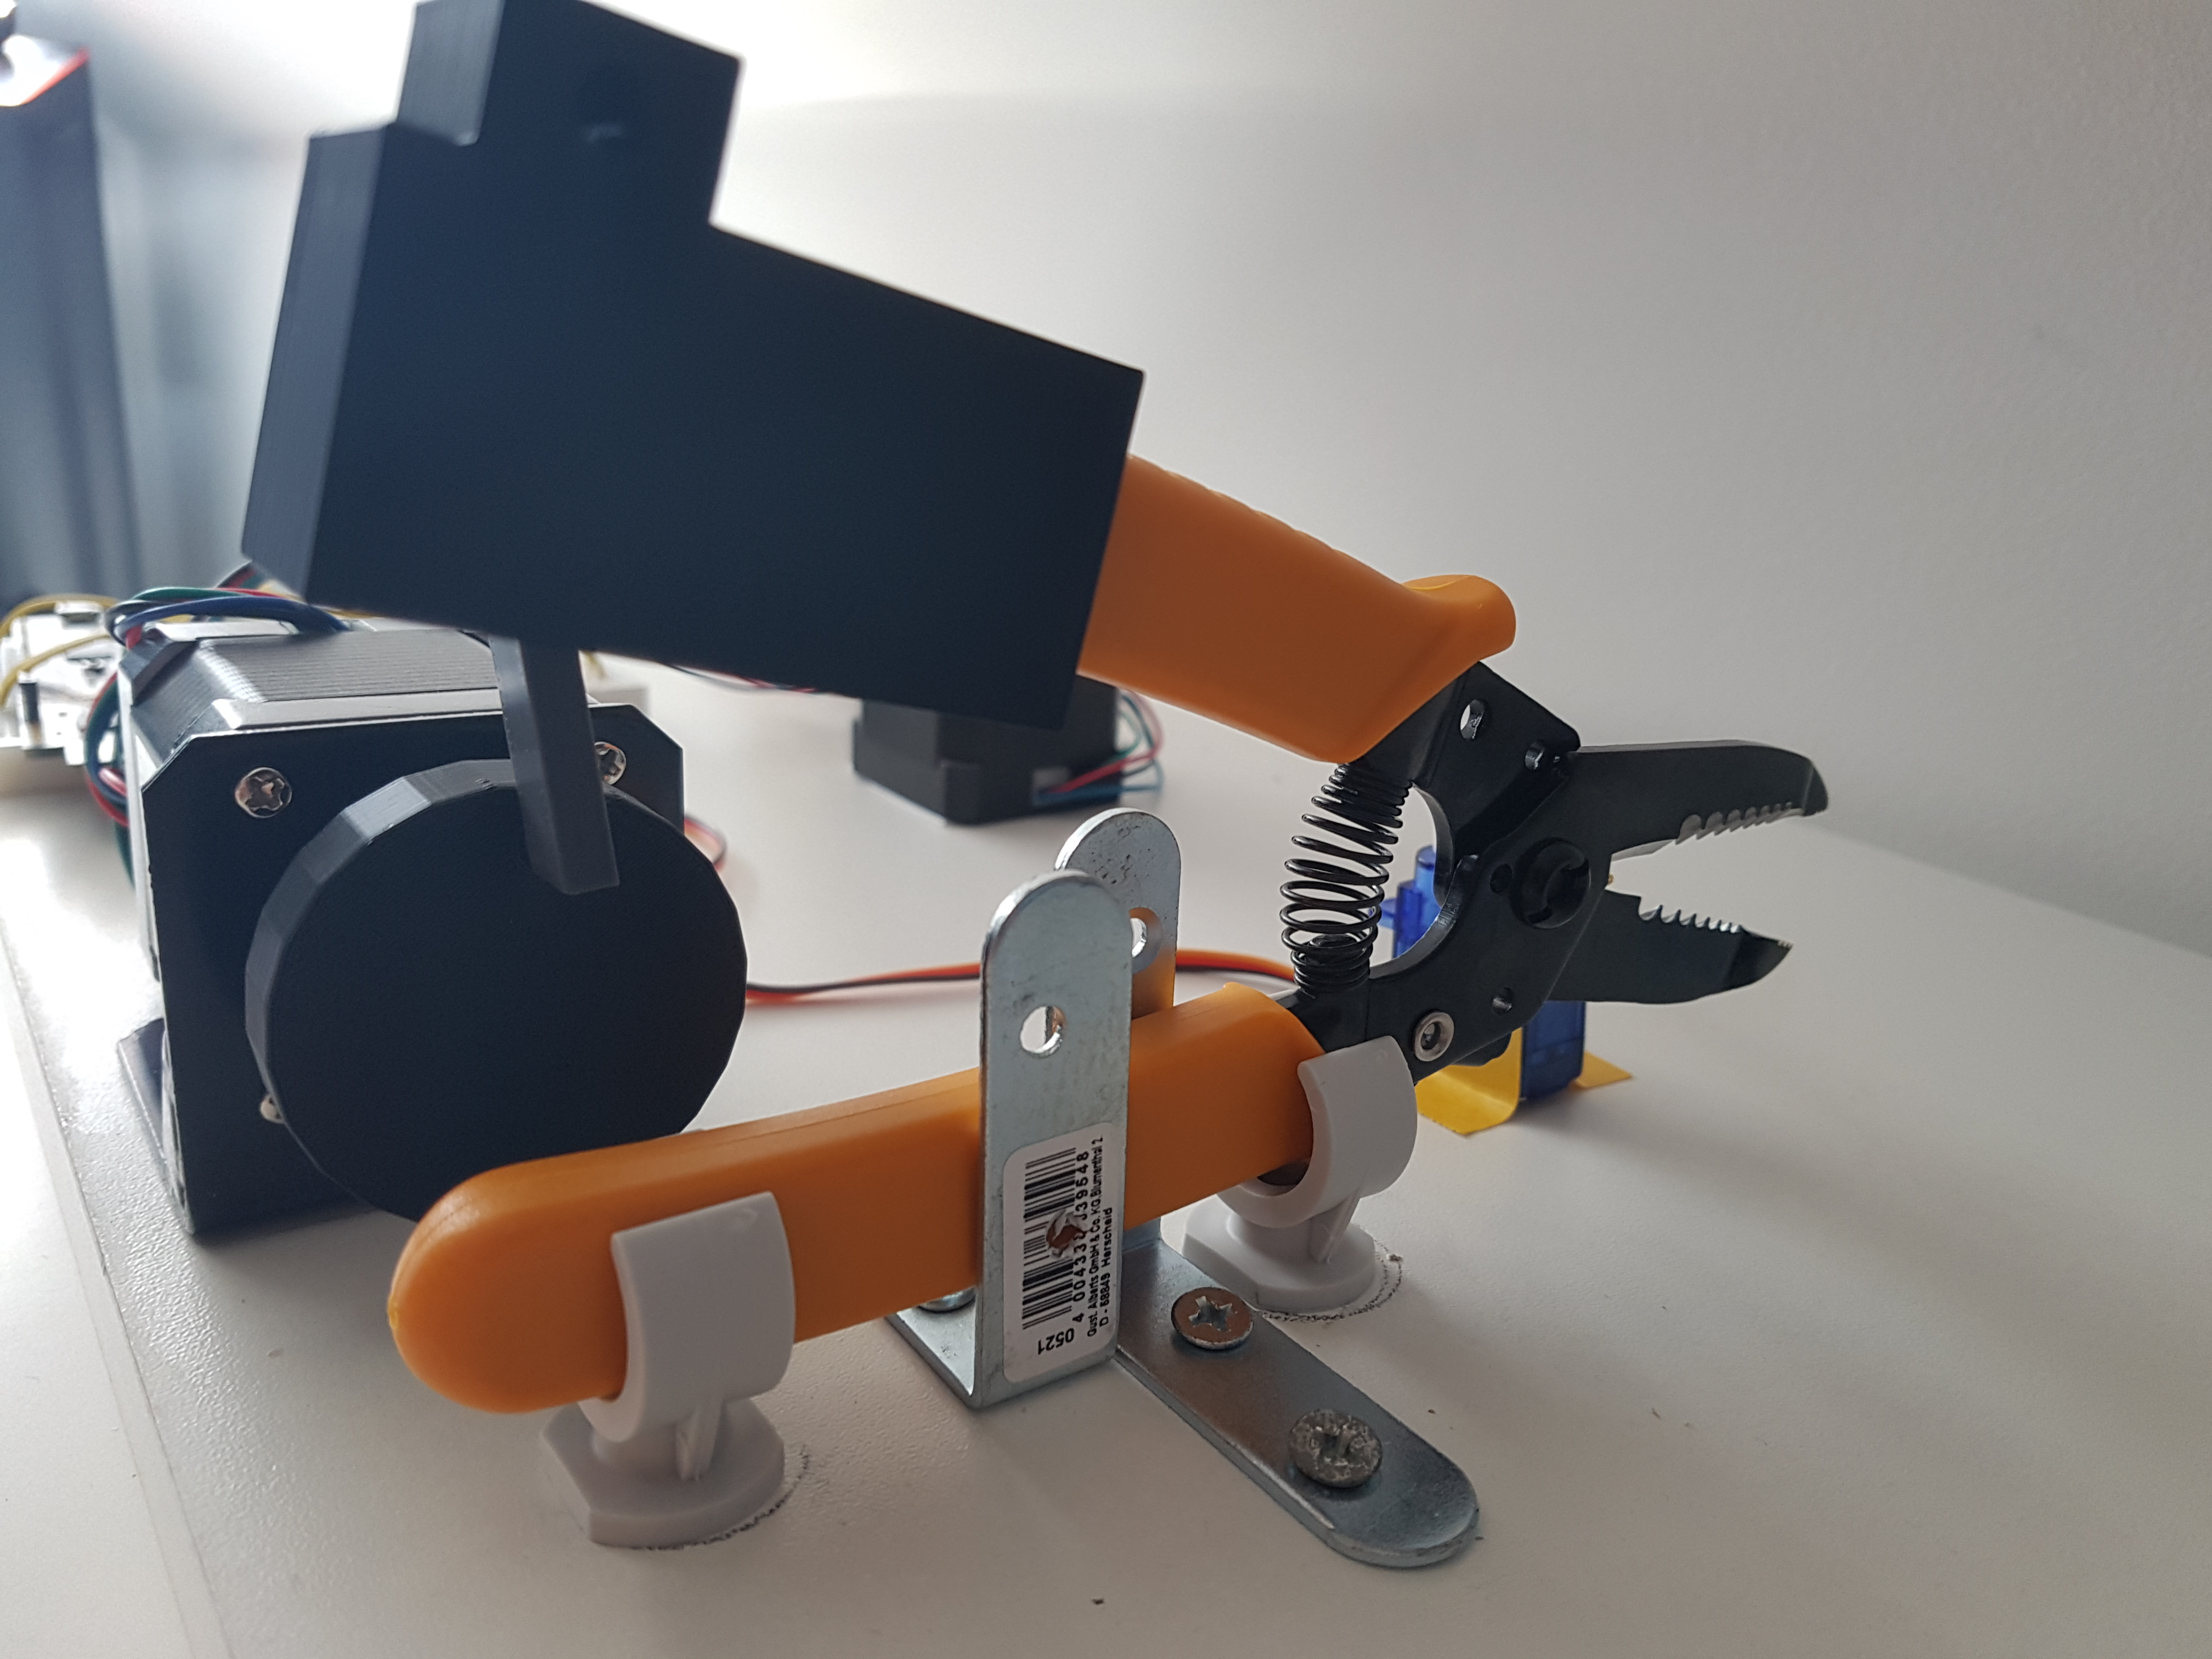
\includegraphics[width=0.65\textwidth]{images/proto2.jpg}
    \caption{Point de vue rapproché sur la pince à dénuder et le système bielle-manivelle}
    \label{fig:proto2}
\end{figure}